\documentclass{article}
\usepackage[spanish]{babel}
\usepackage{amsmath}
\usepackage{amsthm}
\usepackage{amssymb}
\usepackage{ dsfont }
\usepackage{adjustbox}
\usepackage[shortlabels]{enumitem}
\usepackage[margin=1in]{geometry}
\usepackage{caption}
\usepackage[nocheck]{fancyhdr}
\usepackage[most]{tcolorbox}
\usepackage{xcolor}
\usepackage{biblatex}
\usepackage{listings}
\usepackage{algorithm}
\usepackage{algpseudocode}
\usepackage{pgffor}
\usepackage{import}
\usepackage{MnSymbol,wasysym}
\usepackage{graphicx}
\usepackage{float}



\renewcommand{\qedsymbol}{$\blacksquare$}

\addto\captionsspanish{\renewcommand{\proofname}{\normalfont{\textbf{Solución}}}}

\addbibresource{references.bib}

\thispagestyle{fancy}
\rhead{
\includegraphics[scale=0.07]{images/Logo_FC.png}}
\lhead{
\includegraphics[scale=0.065]{images/Logo_FC.png}}
\chead{\large\textbf{Gestión de Inventario y Punto de Venta} \\
\textbf{Facultad de Ciencias - UNAM}\\
\textsc{Ingeniería de Software}\\
\textsc{Febrero 2025}\\
\centering{Un sistema de software para administrar de manera\\ eficiente un comercio.}
}
\renewcommand{\headrulewidth}{1pt}
%\pagenumbering{gobble}
\AtBeginDocument{\vspace*{4.2\baselineskip}}

\definecolor{FireBlue}{rgb}{0,0, 54.5}
\definecolor{Salmon}{rgb}{	80.8, 93.7, 100}

\begin{document}

\tableofcontents

\listoffigures

\section{Base de Datos}

\subsection{Modelo Entidad Relación}

\section{Backend}

\begin{figure}[H]
    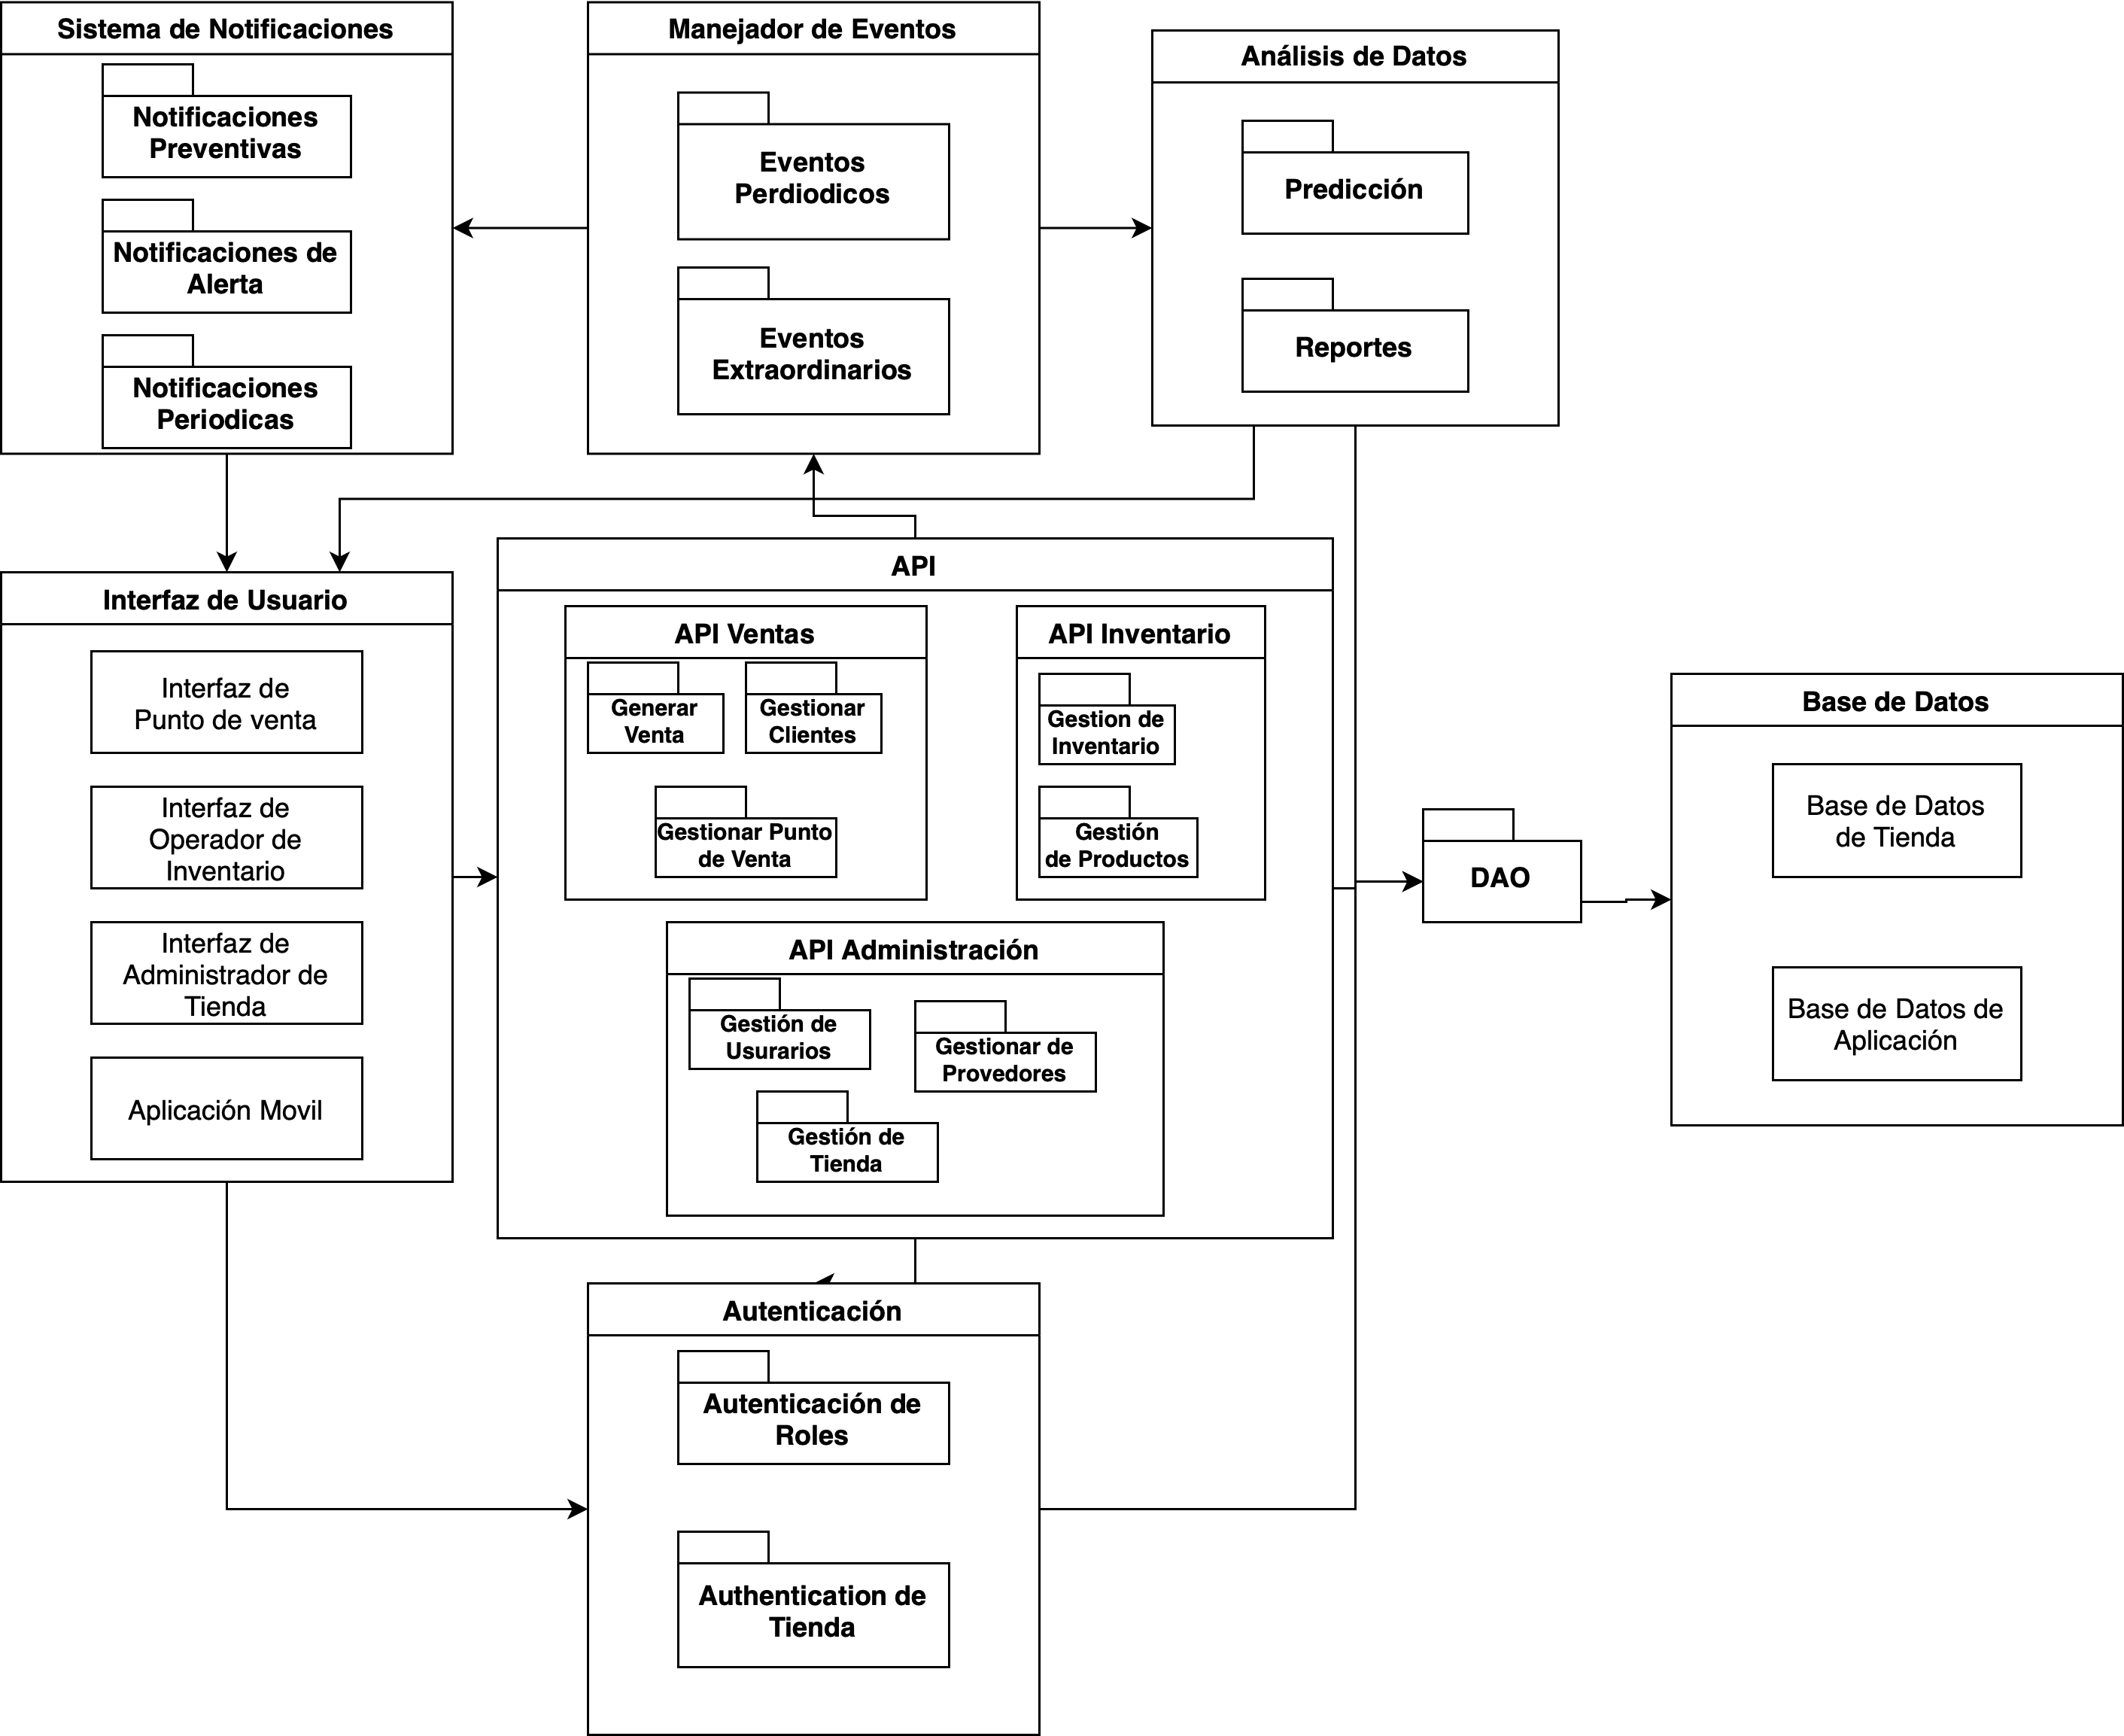
\includegraphics[width=\textwidth]{images/BackEnd.png}
    \centering
    \caption{Arquitectura del Backend de la Aplicación}
\end{figure}

\subsection{DAO}

El DAO (Data Access Object) será el encargado de administrar todos los accesos a la base de datos, permitiendo la interacción entre la aplicación y el almacenamiento de datos de manera estructurada y eficiente.

\subsection{API de Puntos de Venta}

Esta API gestionará las operaciones relacionadas con el punto de venta, permitiendo la generación de ventas, la administración de clientes y la gestión de los puntos de venta.

\subsection{API de Operaciones de Inventario}

Encargada de administrar el inventario de la tienda, permitiendo el control de stock, registro de movimientos de productos y actualización de información de los artículos disponibles.

\subsection{API de Administración de Inventario}

Facilita la gestión de productos y proveedores, asegurando el abastecimiento adecuado de la tienda y la correcta administración de los recursos.

\subsection{Manejador de Eventos}

El manejador de eventos procesará diversas acciones dentro del sistema, tales como ventas, asignaciones de tareas, eventos periódicos y recepciones de inventario. Su función principal es notificar a los módulos correspondientes, en especial al sistema de notificaciones.

\subsection{Sistema de Notificaciones}

El sistema de notificaciones será el encargado de enviar alertas y recordatorios a los destinatarios correspondientes según los eventos que lo activen. Dependiendo del tipo de evento, se generará una notificación específica.

\subsubsection{Notificaciones Periódicas}

Son aquellas notificaciones programadas por el administrador de la tienda para ser enviadas en intervalos regulares, conteniendo información relevante según la configuración establecida.

\subsubsection{Notificaciones Preventivas}

Notificaciones enviadas de manera anticipada en función de los eventos en curso dentro de la tienda, con el objetivo de prevenir posibles incidencias o tomar decisiones estratégicas a tiempo.

\subsubsection{Notificaciones de Alerta}

Se generan ante eventos extraordinarios o críticos que ocurran en la tienda. Estas alertas son enviadas de forma inmediata a los usuarios correspondientes para su pronta atención.

\subsection{Análisis de Datos}

Este módulo se encargará del procesamiento y análisis inteligente de la información disponible en el sistema, permitiendo obtener conocimientos útiles a partir de los datos almacenados.

\subsubsection{Pronósticos}

Proveerá predicciones sobre eventos futuros con base en datos históricos, buscando ofrecer resultados lo más precisos posible.

\subsubsection{Reportes}

Generará informes personalizados según los datos requeridos por el usuario, extrayendo y procesando la información relevante de la base de datos.

\subsection{Autenticación}

Este módulo verificará la identidad de los usuarios y validará sus permisos para acceder a funciones específicas dentro del sistema.

\subsubsection{Autenticación de Roles}

Validará las acciones que un usuario puede realizar dentro de una tienda específica, asegurando que solo accedan a las funcionalidades autorizadas.

\subsubsection{Autenticación de Tienda}

Se encargará de validar el acceso a una tienda determinada, asegurando que el usuario tenga los permisos necesarios para ingresar a la misma.


\section{Vistas}

Aquí se presentan las vistas que contendrá la aplicación para la interacción con el usuario.

\subsection{Inicio de Sesión}

\begin{figure}[H]
    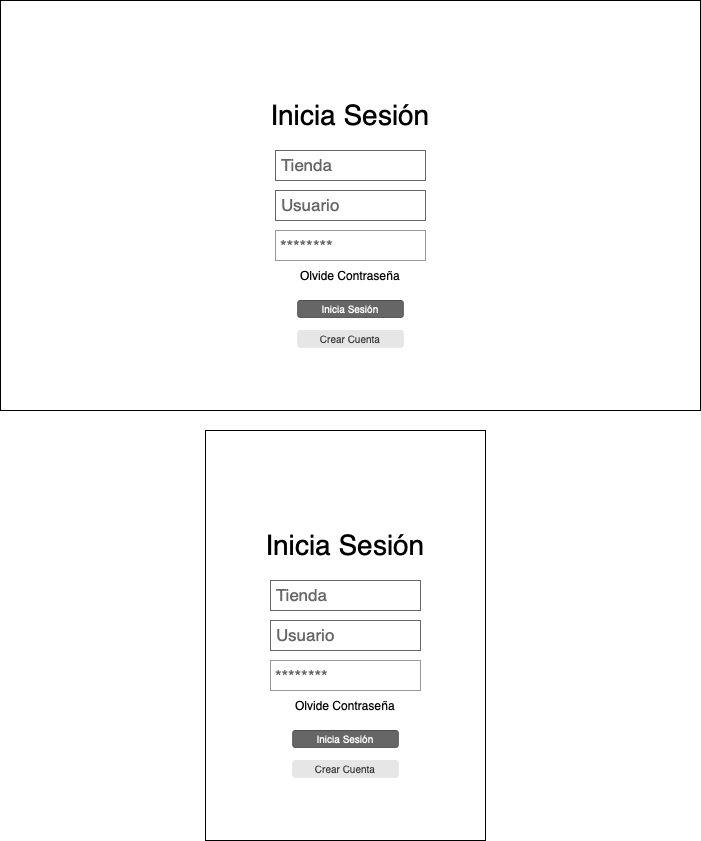
\includegraphics[width=.75\textwidth]{images/InicioSesion.png}
    \centering
    \caption{Página de inicio de sesión en web y vista de cliente Android.}
\end{figure}

La pantalla de inicio de sesión permite a los usuarios autenticarse en la aplicación ingresando sus credenciales.
En la versión web y móvil, se presenta un diseño simple con campos para usuario y contraseña, así como opciones para 
recuperar el acceso en caso de olvido.


\subsection{Crear Cuenta}

\begin{figure}[H]
    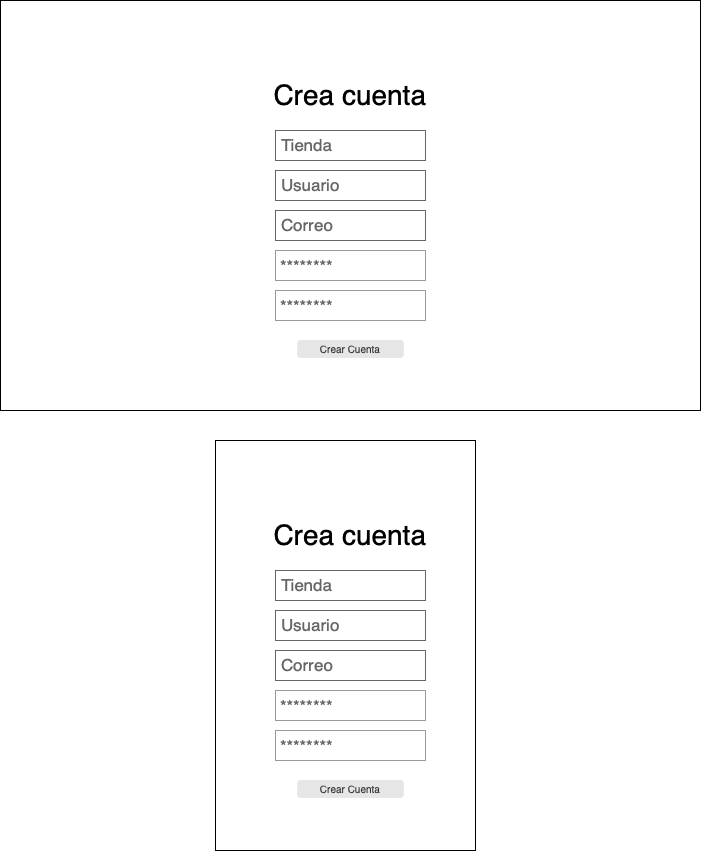
\includegraphics[width=.75\textwidth]{images/CreaCuenta.png}
    \centering
    \caption{Página para la creación de una cuenta en web y vista en cliente Android.}
\end{figure}

La interfaz de creación de cuenta permite a los nuevos usuarios registrarse proporcionando su información básica.
Se incluyen campos para nombre, correo electrónico, contraseña y nombre de tienda.

\subsection{Página de Inicio}

\begin{figure}[H]
    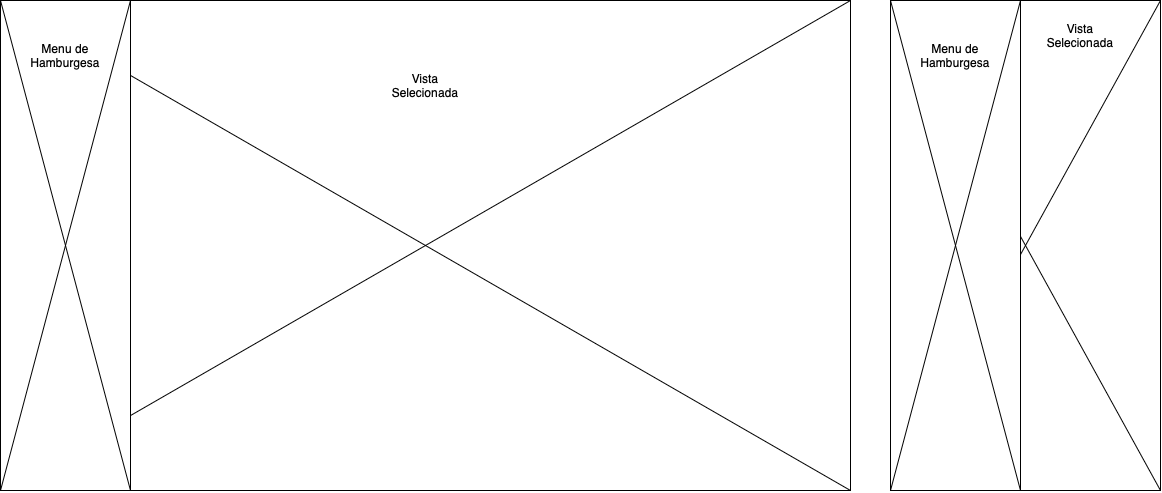
\includegraphics[width=.75\textwidth]{images/Inicio.png}
    \centering
    \caption{Página de inicio de la aplicación web y su contraparte en cliente Android.}
\end{figure}

Desde la página de inicio, los usuarios pueden navegar a las diferentes secciones de la aplicación. Contiene un menú de
hamburguesa que da acceso a las funcionalidades principales, como ventas, inventario, reportes y administración dependiendo el caso.

\subsection{Punto de Venta}

\begin{figure}[H]
    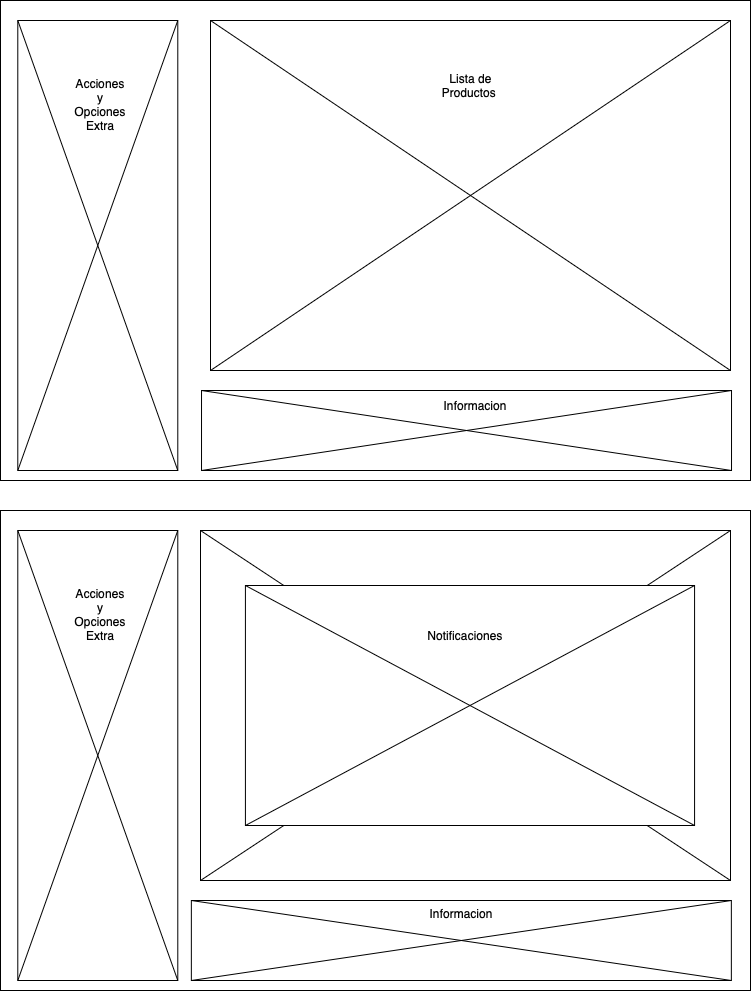
\includegraphics[width=.75\textwidth]{images/POS.png}
    \centering
    \caption{Página del punto de venta en web con notificación emergente.}
\end{figure}

La interfaz del punto de venta permite registrar ventas en tiempo real. Cuenta con un menú de hamburguesa para acceder
a funciones adicionales y una sección central donde se muestran los productos agregados al ticket.
En la parte inferior, se visualiza información relevante como cupones, descuentos y el total de la venta.
Además, pueden aparecer notificaciones emergentes para alertar al usuario sobre eventos importantes.

\subsection{Administración}

\begin{figure}[H]
    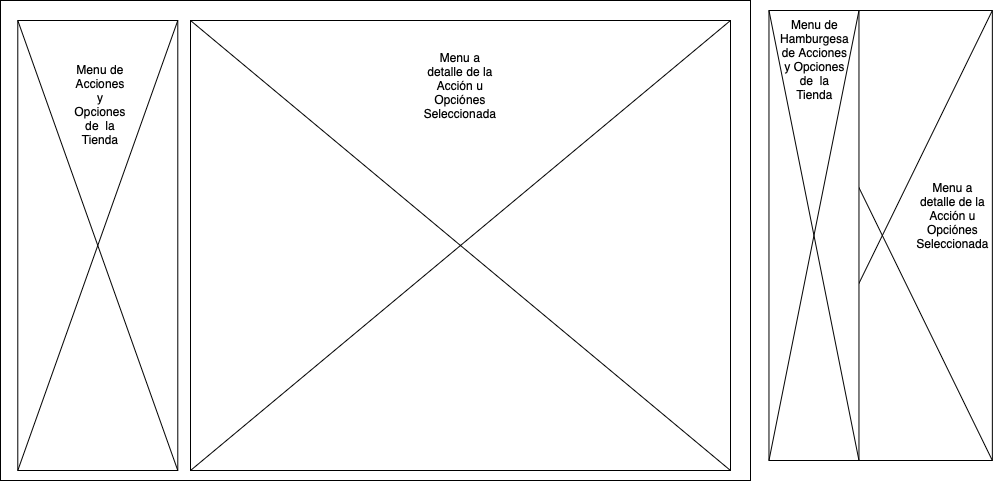
\includegraphics[width=.75\textwidth]{images/Administracion.png}
    \centering
    \caption{Página de administración de la tienda en web con su contraparte en el cliente Android.}
\end{figure}

La sección de administración permite gestionar usuarios, permisos y configuraciones generales de la tienda.
Presenta un menú de hamburguesa que facilita la navegación entre las distintas opciones de configuración.

\subsection{Manejo de Inventario}

\begin{figure}[H]
    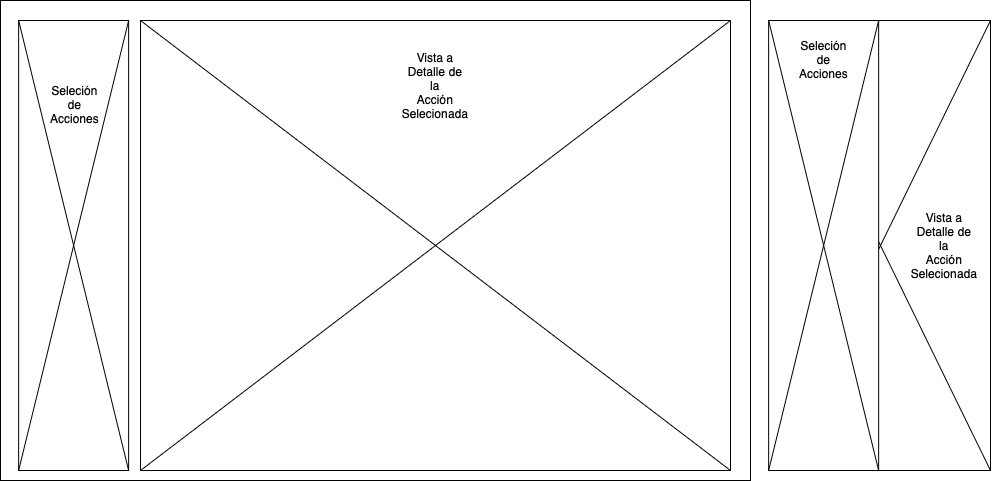
\includegraphics[width=.75\textwidth]{images/Inventario.png}
    \centering
    \caption{Página para el manejo del inventario de la tienda en web y en su vista Android.}
\end{figure}

Desde esta sección, los usuarios pueden gestionar el stock de productos, actualizar información de artículos
y realizar ajustes en el inventario. El menú de hamburguesa permite acceder a opciones como control de existencias
y gestión de proveedores.

\subsection{Análisis de Datos y Reportes}

\begin{figure}[H]
    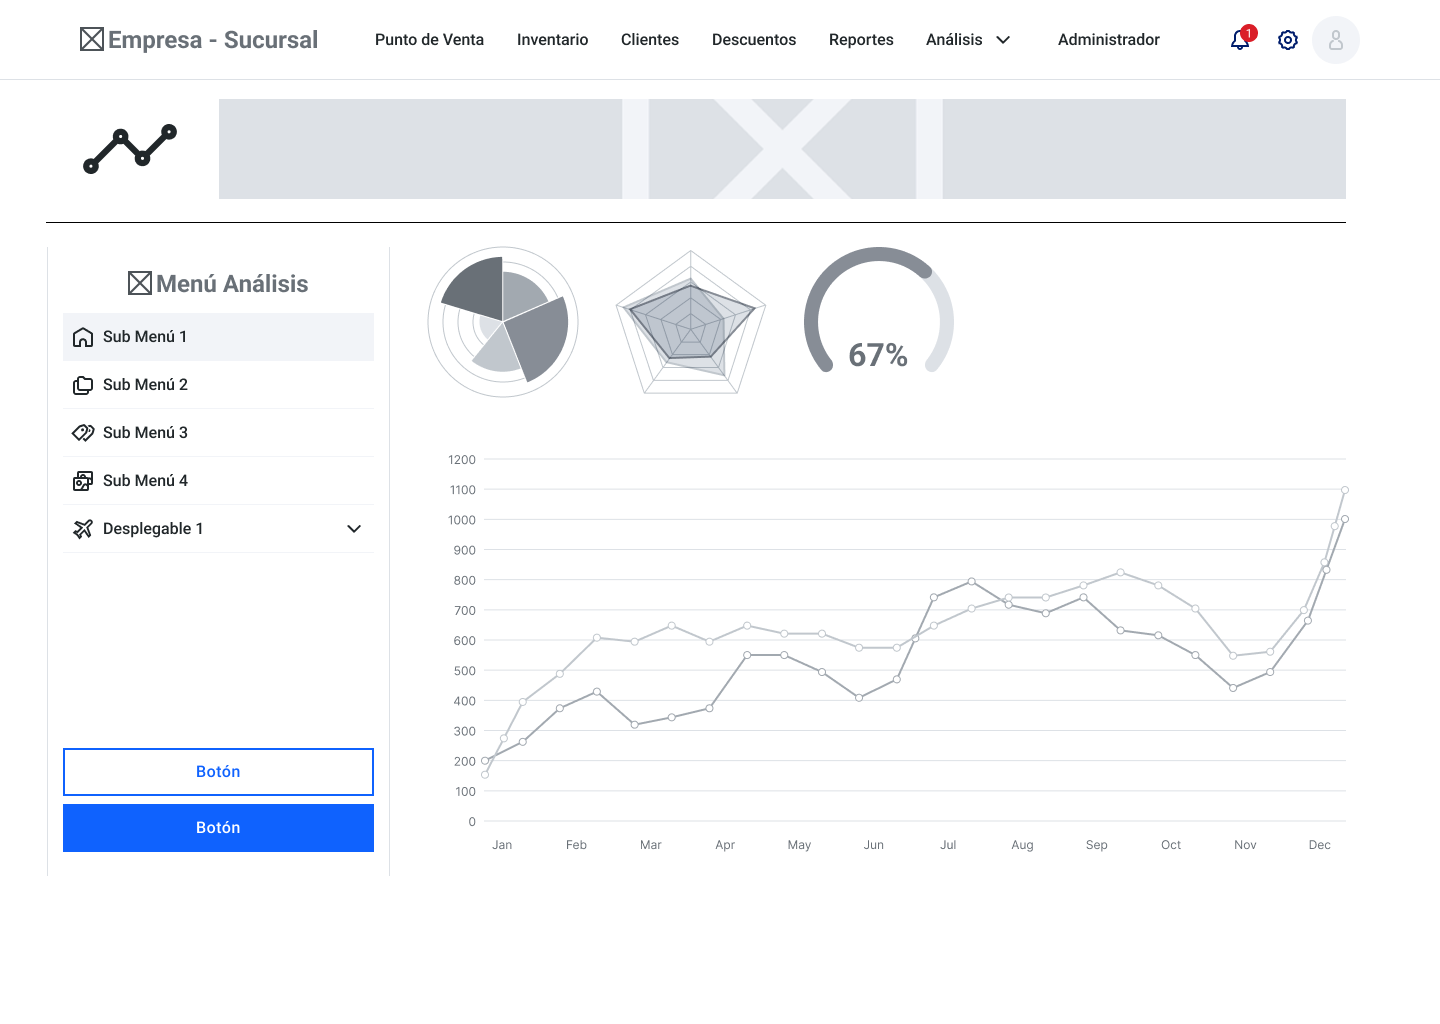
\includegraphics[width=.75\textwidth]{images/Analisis.png}
    \centering
    \caption{Página para la consulta de análisis y reportes en web y su vista correspondiente en Android.}
\end{figure}

Esta sección permite visualizar reportes y realizar análisis de datos basados en el historial de ventas e inventario.
A través del menú de hamburguesa, el usuario puede seleccionar entre generación de reportes y herramientas de predicción
de tendencias.


\end{document}